\usetikzlibrary{arrows.meta,calc,positioning}
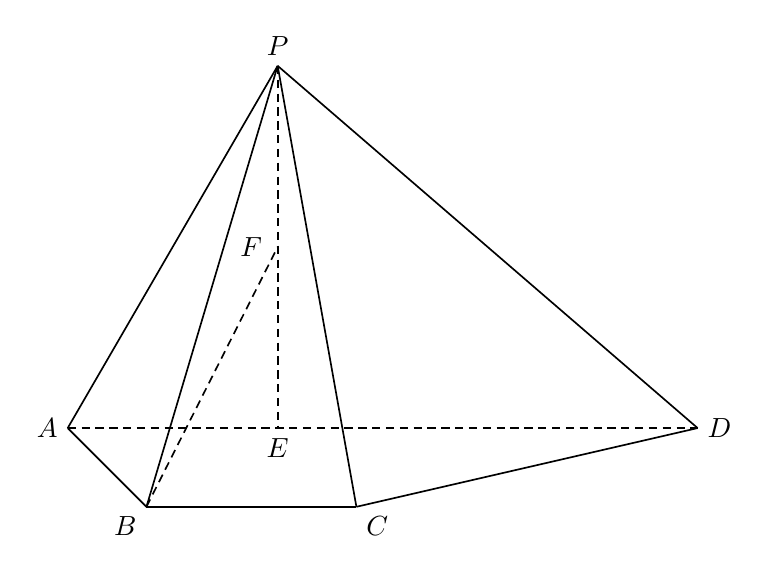
\begin{tikzpicture}[x=1cm,y=1cm,line width=.6pt,font=\normalsize,>=Stealth]
% 2024_beijing_q17: pyramid P-ABCD, E on AD, F on PE
\coordinate (P) at (-1.333333333,4.6);
\coordinate (A) at (-4.0,0);
\coordinate (E) at (-1.333333333,0);
\coordinate (D) at (4.0,0);
\coordinate (B) at (-3.0,-1.0);
\coordinate (C) at (-0.3333333333,-1);
\coordinate (F) at (-1.333333333,2.3);
% solid lateral + base front
\draw[solid] (P)--(A);
\draw[solid] (P)--(B);
\draw[solid] (P)--(C);
\draw[solid] (P)--(D);
\draw[solid] (A)--(B);
\draw[solid] (B)--(C);
\draw[solid] (C)--(D);
% hidden
\draw[densely dashed] (A)--(D);
\draw[densely dashed] (P)--(E);
\draw[densely dashed] (B)--(F);
% labels
\node[above] at (P) {$P$};
\node[left] at (A) {$A$};
\node[below left] at (B) {$B$};
\node[below right] at (C) {$C$};
\node[right] at (D) {$D$};
\node[below] at (E) {$E$};
\node[left,xshift=-2pt] at (F) {$F$};
\end{tikzpicture}
